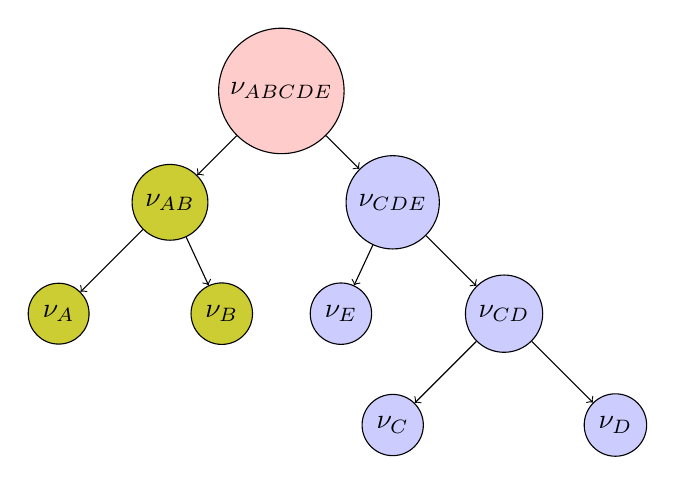
\begin{tikzpicture}
\tikzset{classA/.style={circle, draw=black, fill=blue!20!yellow}, node distance=2cm}
\tikzset{classB/.style={circle, draw=black, fill=blue!20}, node distance=2}
\tikzset{classX/.style={circle, draw=black, fill=red!20}, node distance=2cm}
\uncover<1->{
\node[classX] (ABCDE) {$\nu_{ABCDE}$};}
\uncover<2->{
\node[classA, below left of=ABCDE] (AB) {$\nu_{AB}$};
\node[classB, below right of=ABCDE] (CDE) {$\nu_{CDE}$};}
\uncover<5->{
\node[classA, below left of=AB] (A) {$\nu_A$};
\node[classA, below right of=AB, xshift=-5ex] (B) {$\nu_{B}$};}
\uncover<3->{
\node[classB, below left of=CDE, xshift=5ex] (E) {$\nu_E$};
\node[classB, below right of=CDE] (CD) {$\nu_{CD}$};}
\uncover<4->{
\node[classB, below left of=CD] (C) {$\nu_{C}$};
\node[classB, below right of=CD] (D) {$\nu_{D}$};
}
\uncover<2->{
\draw[->] (ABCDE)--(AB);
\draw[->] (ABCDE)--(CDE);
}
\uncover<5->{
\draw[->] (AB)--(A);
\draw[->] (AB)--(B);
}
\uncover<3->{
\draw[->] (CDE)--(E);
\draw[->] (CDE)--(CD);
}
\uncover<4->{
\draw[->] (CD)--(C);
\draw[->] (CD)--(D);
}
\end{tikzpicture}
